\documentclass{article}
\usepackage[margin=2cm, headheight=0pt, headsep=1cm, includeheadfoot, top=0.75cm, bottom=1cm]{geometry}
\usepackage{enumerate, fancyhdr, graphicx, amsmath, float, url, hyperref, color}
\usepackage{array,booktabs,dirtree,subcaption,nameref}

\title{Vault 5431 - Design}
\author{Paul Chesnais, Alicia Wu, Britney Wong, Chang Yang Jiao}
\date{\today}

\pagestyle{fancy}
\fancyhead{}
\lhead{pmc85, yw344, bmw227, cj285}
\chead{Vault 5431 - Sprint Report}
\rhead{\today}
\fancyfoot{}
\rfoot{\thepage}
\lfoot{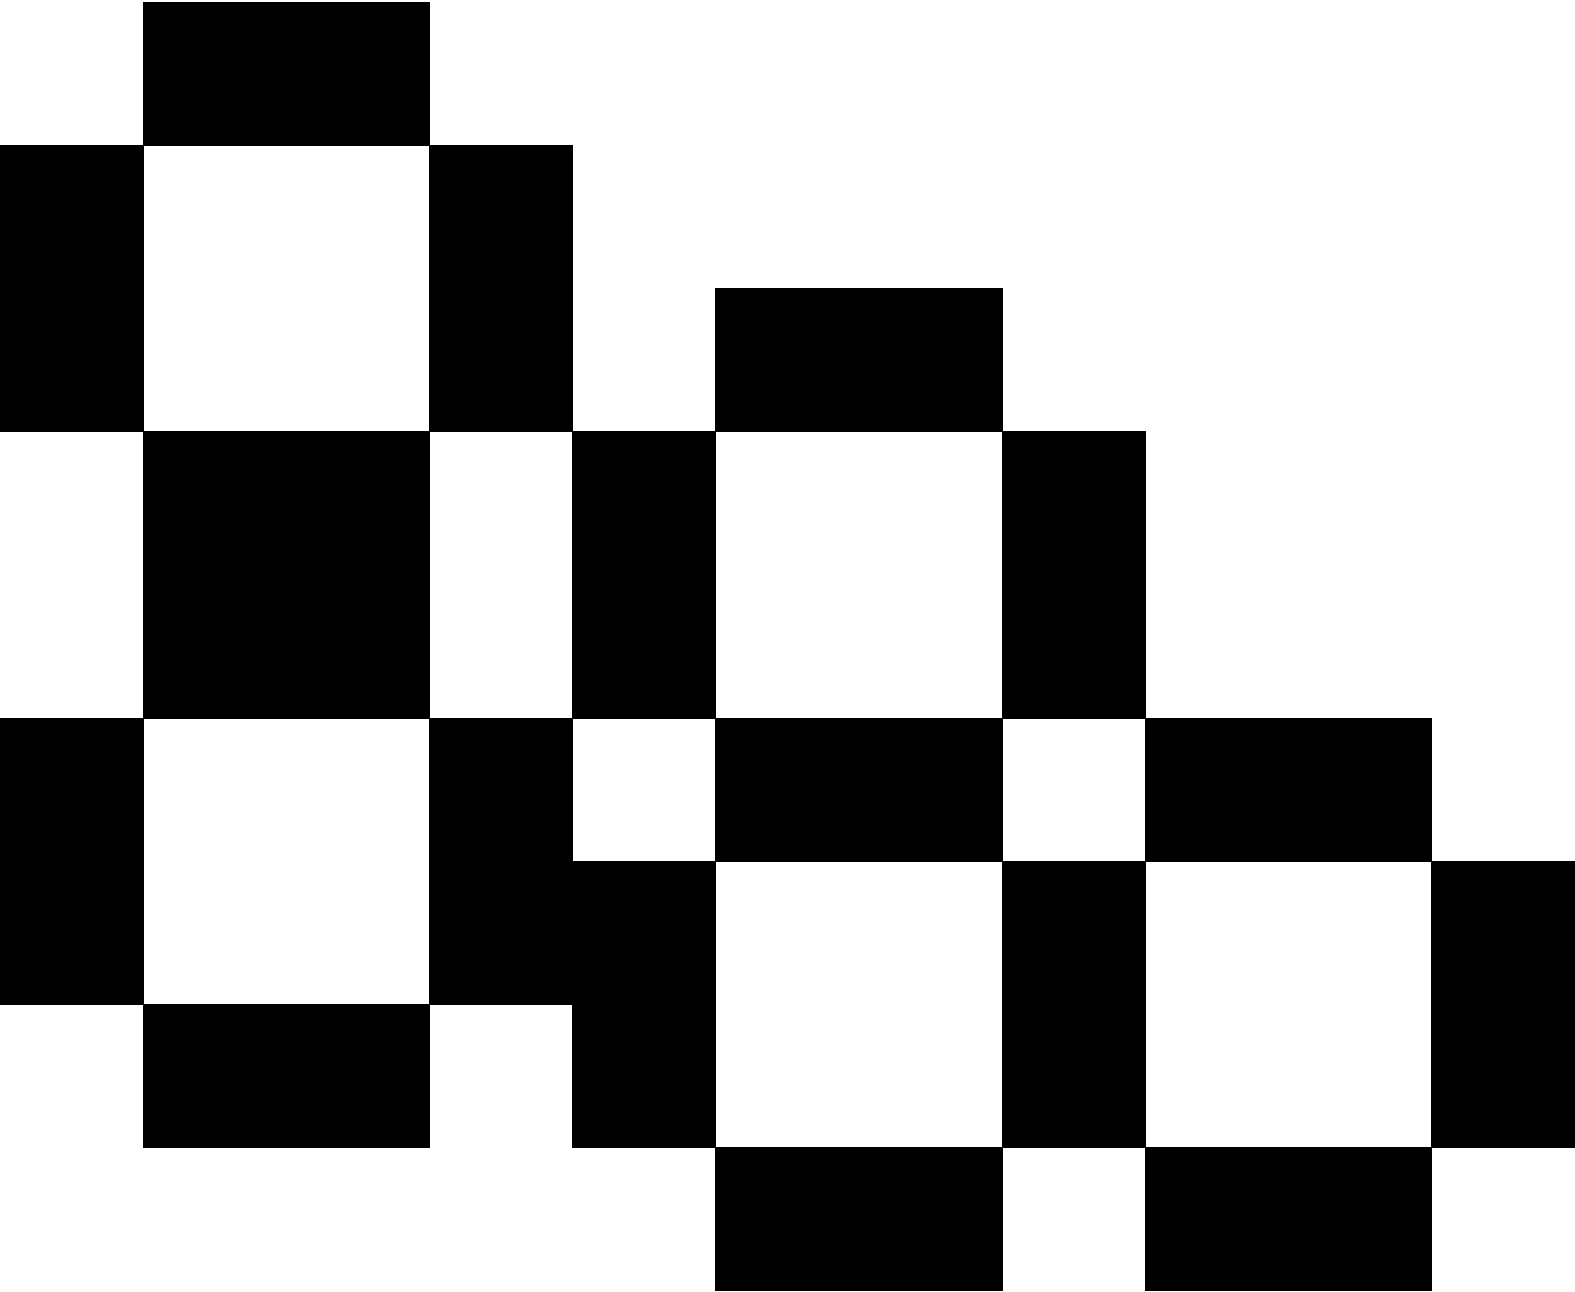
\includegraphics[height=20pt]{figures/Logo}}
\renewcommand{\headrulewidth}{0.5pt}
\renewcommand{\footrulewidth}{0.5pt}

\usepackage{listings, color, times, textcomp, setspace}
\definecolor{Code}{rgb}{0,0,0}\definecolor{Decorators}{rgb}{0.5,0.5,0.5}\definecolor{Numbers}{rgb}{0.5,0,0}
\definecolor{MatchingBrackets}{rgb}{0.25,0.5,0.5}\definecolor{Keywords}{rgb}{0,0,1}\definecolor{self}{rgb}{0,0,0}
\definecolor{Strings}{rgb}{0,0.63,0}\definecolor{Comments}{rgb}{0,0.63,1}\definecolor{Backquotes}{rgb}{0,0,0}
\definecolor{Classname}{rgb}{0,0,0}\definecolor{FunctionName}{rgb}{0,0,0}\definecolor{Operators}{rgb}{0,0,0}
\definecolor{Background}{rgb}{0.98,0.98,0.98}

\lstdefinestyle{Pseudocode}{
  backgroundcolor=\color{Background},basicstyle=\ttfamily\small\setstretch{1},breaklines=true,mathescape,language=Java,
  commentstyle=\color{Comments}\slshape,emph={self},emphstyle={\color{self}\slshape},frame=l,framexbottommargin=2em,
  framextopmargin=2em,keywordstyle={[2]\color{Numbers}},keywordstyle={\color{Keywords}\bfseries},
  morekeywords={for,while,if,in,else,break,def,not,return,and,or,execute,on,record},otherkeywords={->},
  morekeywords=[2]{Sign,Verify,Enc,Dec,AuthEnc,AuthDec,H,PBKDF2},
  numbers=left,numbersep=1em,numberstyle=\footnotesize,showspaces=false,showstringspaces=false,showtabs=false,
  stringstyle=\color{Strings},tabsize=4,xleftmargin=1em,
}
\lstMakeShortInline[columns=fixed,style=Pseudocode]|
\renewcommand{\lstlistingname}{Protocol}

\begin{document}
\maketitle
\thispagestyle{empty}

\section{Server Environment}
\label{sec:server_environment}

\subsection{Platform}
\label{sub:platform}
\par The server is running Ubuntu 15.10 with weekly backups. SSH access is only allowed for SysAdmins whose keys have been cleared, with password login disabled.

\subsection{Server Startup}
\label{sub:server_startup}
\par The first thing to do is to start the VaultRedirector server, which simply listens to all HTTP requests coming on port 80 and redirects to ``/'' on port 443 (dropping all of the request's contents in the process). This is to force users to use HTTPS and prevent them from accidentally sending information via an insecure channel.
\par Next, the Vault server needs to be started up. The program requires access to three files: the \texttt{/root/.vault5431/} directory that stores all of the required data (see \nameref{sub:filesystem_design}), the Java KeyStore \texttt{keystore.jks} that contains the encrypted private key for the SSL certificate and the KeyStore \texttt{truststore.jks} that contains manually trusted certificates for the SMS messaging service. Upon startup, the program prompts the SysAdmin for three passwords: the admin password, from which the Admin Signing Key (ASK), the Admin Encryption Key (AEK) and the Admin Logging Key (ALK) are derived, the password under which the SSL certificate's private key is encrypted and the password used to verify the trust store's authenticity. The Admin password is only known to the four members of the team.
\par Protocol~\ref{lst:admin_key_derivation} describes how the Admin Keys are generated from the admin password. The password is read from the console into the \texttt{adminPassword} array. This array is zeroed out after the keys have been generated, in the hopes that this will decrease the likelihood of it ending up on disk. If the system was never initialized, it will generate a random 32 byte salt and save it under \texttt{/root/.vault5431/admin.salt}. The salt is required for PBKDF2, and therefore needs to stay constant throughout, otherwise the Admin Keys will not stay the same after restart. The salt is then read into the \texttt{salt} array.
\begin{lstlisting}[caption={Admin Key Derivation},label={lst:admin_key_derivation},style=Pseudocode]
adminPassword = adminPassword $\oplus$ 'e' // e for encryption
AEK = PBKDF2(adminPassword, salt)
adminPassword = adminPassword $\oplus$ 'e' // back to original password
adminPassword = adminPassword $\oplus$ 's' // s for signing
ASK = PBKDF2(adminPassword, salt)
adminPassword = adminPassword $\oplus$ 's' // back to original password
adminPassword = adminPassword $\oplus$ 'l' // l for logging
ALK = PBKDF2(adminPassword, salt)
\end{lstlisting}
\par Finally, each User acquires their own set of encryption (UEK), signing (USK) and logging (ULK) keys, all derived from the respective Admin Keys. They are in no way more secret than the Admin Keys, but they serve the purpose of encrypting and signing each log under different keys, along with other User settings and data. The User Keys are simply derived by hashing the User's username along with the respective Admin Key. Please refer to the \nameref{sub:user_creation} section to see how the User Keys are derived.

\subsection{Filesystem Design}
\label{sub:filesystem_design}

\begin{figure}[h!]
  \centering
  \begin{subfigure}[b]{0.3\textwidth}
    \dirtree{%
      .1 .vault5431/.
      .2 (username hash).
      .3 crypto.priv.
      .3 crypto.pub.
      .3 log.
      .3 password.hash.
      .3 settings.
      .3 shared.
      .3 signing.priv.
      .3 signing.pub.
      .3 vault.
      .3 vault.salt.
      .2 log.
      .2 admin.salt.
    }
  \end{subfigure}
  \caption{Directory Structure}
  \label{fig:directory_structure}
\end{figure}

\par All of the relevant data are stored in a directory called \texttt{.vault5431} in server's root. All of a given user's information and data is stored in their respective sub-directories. The system log is stored in \texttt{.vault5431/log}, and the salt used to derive the Admin Keys is stored in \texttt{.vault5431/admin.salt}.
\par Please refer to the \nameref{sub:user_creation} section for a detailed explanation of what is contained in each file.

\subsection{Rationale}
\par We decided to use a filesystem design over a database for two main reasons. First, it immediately prevents SQL injections from occurring, which is one less thing our system needs to worry about. Second, it makes it simpler to manage encryption of and signatures for individual files, which we will be extensively using to ensure the integrity and confidentiality of the user data.

\section{Audit}
For the audit section of our project, we organized our logs based on two types- the user logs and the system log.
\subsection{Tamperproof Logging}
\par All logs in this system follow a tamperproof logging scheme. Here is the protocol for tamperproof logging \cite{bib:TamperProof}, as defined in class:
\begin{lstlisting}[caption={Tamperproof Logging},label={lst:tamperproof_logging},style=Pseudocode]
ek = H("encrypt", ULK)
x = AuthEnc(m; ek; ULK)
record x in log
ak = H("iterate", ak)
\end{lstlisting}
Both user specific logs and the system log are encrypted and signed under this scheme, using their respective keys.

\subsection{User Logs}
\par All the information in our system is organized in a file system structure. Therefore, each user has his own directory containing his log files, password files, keys, and other information found in his vault. Each user log entry has five fields: the log level (debug, info, warning, or error), the IP address that completed the specified action, the hashed username, the timestamp of when the action was initiated, and the message that specifies the type of action that took place. The Vault username is hashed to prevent a user's username from being discovered in the case where an attacker somehow manages to get the log. We believe that because it is reasonable for a user to use same username in multiple places (to reduce memorization burden), an attacker should not be able to discover a username even if he successfully attacks our system.

\par Currently, a log entry is created when a new password is created, a password is viewed, a password is modified, when a password is modified, or when passwords are shared and accepted. Furthermore, changes in settings will be logged. Additionally, both successful or failed logins are also logged.

\par Finally, a user can currently see his personal log by successfully logging into his account and clicking on the log link on their dashboard. From there, he will be able to see each log entry with four fields – the log type, the IP address, timestamp, and message with the action. The signature validation validation now takes place behind the scene.

% when it is implemented, will be done behind the scenes before the log is displayed.

\subsection{System Log}
The system log should only be viewed by the admins of our system (the four of us). We will have our own system keys to be able to access the system log, and the system log entry fields are the same as for the user log. We create log entries for actions done by the server, as well as log entries for error events (ex: unsuccessful login events, user creation, etc.), so we have the information to recognize a potential attack on our system.

\section{Authentication}

\subsection{User Creation}
\label{sub:user_creation}
\par In order to create a new account, the Client must provide the following parameters:
\begin{description}
  \item[\texttt{username}] The desired username.
  \item[\texttt{hashedPassword}] The User's master password hashed with the string ``auth'', i.e. |H("auth", masterPassword)|.
  \item[\texttt{phoneNumber}] The desired phone number on which to receive 2FA text messages.
  \item[\texttt{pubCryptoKey}] A public ElGamal key.
  \item[\texttt{privCryptoKey}] The respective private ElGamal key, encrypted under |H(masterPassword)|
  \item[\texttt{pubSigningKey}] A public ECDSA key.
  \item[\texttt{privSigningKey}] The respective private ECDSA key, encrypted under |H(masterPassword)|.
\end{description}
\par All of the Elliptic Curve keys lie on the NIST P-384 curve. Protocol~\ref{lst:user_creation_protocol} defines how a User is created. Only one User can be created at a time, and Protocol~\ref{lst:user_creation_protocol} is only run if there exists no directory in \texttt{/root/.vault5431} named |H(username)|. If no such directory exists, it is created and assigned to the User. On the other hand, if the directory exists, it means the username is already taken, and the User will be notified. There is no way to completely prevent an attacker from knowing if a username is a valid one in our system or not because they will be notified on sign up.
\begin{lstlisting}[caption={User Creation Protocol},label={lst:user_creation_protocol},style=Pseudocode]
h := H(username)
UEK := H(h, AEK)
USK := H(h, ASK)
ULK := H(h, ALK)
record PBKDF2(hashedPassword, randomSalt()) in password.hash
record Sign(h + pubCryptoKey; USK) in crypto.pub
record privCryptoKey in crypto.priv
record Sign(h + pubSigningKey; USK) in signing.pub
record privSigningKey in signing.priv
record AuthEnc(phoneNumber; UEK; USK) in settings
record AuthEnc(randomSalt(); UEK; USK) in vault.salt
record $\texttt{\O}$ in log
record $\texttt{\O}$ in vault
record $\texttt{\O}$ in shared
\end{lstlisting}
\par The public keys are signed with the username of the User they belong to prevent an attacker with access to disk from swapping out the public keys and causing all subsequently shared passwords to be encrypted under a key for which they know the private key. An empty log file is created and encrypted under the user's ULK. An empty vault file is created, to contain the encrypted data given by the user, along with an empty shared passwords file. The random salt contained in \texttt{vault.salt} is required for the Client to create the final master encryption key under which all of the passwords will be encrypted. This is to make decrypting a User's vault required both the system's authorization and the client's master password. The User's phone number is saved along with default settings to \texttt{settings}.

\subsection{Client-Side Authentication}
\par The authentication happens in two steps. First, the user is required to type in their username and password. Afterwards, an authentication code will be sent to the user's cellphone as an SMS and the input of this code will be required to access the user vault. Below, each step is explained in greater detail.

\subsubsection{Username and Password}
\par The client sends the username and the hash of the password the server, while storing the first hash of just the password in the browser's Session Storage \cite{bib:session_storage}. The server runs PBKDF2 on the password to verify that it is indeed the correct password. If so, the user is assigned an unverified token (see below). Otherwise, the user is redirected to the login page; after 3 incorrect attempts, the user will be locked out for a period of time. The reason the first hash of the master password in the Session Storage instead of the plaintext is because the session storage is readily available for all to see simply by checking the resources in the web browser. Quite obviously, we do not want the master password to be publicly displayed. We send |H("auth", masterPassword)| to the server instead of |H(H(masterPassword))| because if an attacker finds a target's computer logged in, they can change the master password to whatever they want without knowing the actual master password by presenting the Server with the hash of what is stored in the Session Storage.

\subsubsection{Two Factor Authentication (2FA)}
\par Along with responding with an unverified Token, the Server will also send the User a 6 digit code with a 1 minute expiration time. The point of this code is to authenticate an user based on something that they have (the code, and thus their SMS-receiving phone) in addition to something that they know. This ensures that even if an attacker somehow cracked the User's master password, they still would not have access to the vault. We assume that the User's phone is safely within his/her hands. A user can attempt to verify a 2FA code at most 3 times, after which they will be temporarily banned from logging in. This does not void currently active Tokens. If the user correctly enters the 6 digit code, their Token is upgraded to a verified Token (see below), and they are able to view their vault.

\subsubsection{Decrypting the Vault}
After the user successfully completes 2FA and has received a verified Token, the System sends the Client the encrypted vault along with the decrypted vault salt. To create the final master key, the Client simply computes |H(H(masterPassword, salt)|. This key will be used to encrypt and decrypt the passwords. In this case, the hashing function is SHA-256. SHA-256 is cryptographically strong and remains to be broken, therefore the only way to arrive at the final master key is to know the master password.

\section{Authorization}

\subsection{Tokens for Access Control}
\label{sub:tokens}
\par Once a user has been authenticated (see below), the Reference Monitor assigns them a Token. A Token in this system is the equivalent of a capability. In other words, when the Client presents a valid Token to the Server, the Server can be certain that the User has been authenticated. The Access Control policy is mandatory: Users have access to their own files, and the public keys of all other users in the System (provided that they know their username), but cannot change said access rights. Incidentally, these rights never change; therefore the capability does not need to contain a list of files and their respective rights, rather just the User to whom it was assigned and therefore the files this capability grants access to.

\subsubsection{Body of a Token}
\label{ssub:body_of_a_token}
\par The Tokens used in this system were inspired by JSON Web Tokens (see RFC 7519\cite{bib:RFC7519}), but modified to better suit the system. Here are the fields contained in the Token:
\begin{description}
  \item[\texttt{username}] The User whose files this Token grants access to.
  \item[\texttt{creationDate}] A timestamp indicating when the Token was created by the system.
  \item[\texttt{expiresAt}] When the Token should automatically expire. Users get to choose how long they want their Tokens to last, with a maximum Token time to live of 24 hours.
  \item[\texttt{id}] The Token's unique identifier, here implemented as 128 bit UUIDs generated from a SecureRandom instance.
  \item[\texttt{verified}] Boolean indicating whether or not the User has gone through 2FA, and therefore if this Token allows access to anything other than the 2FA page.
  \item[\texttt{signature}] The signature of the concatenation of the above fields under the current Rolling Key (see below).
\end{description}

\subsubsection{Rolling Keys}
\label{ssub:rolling_keys}
\par Every night, at midnight EST, the server changes signing keys. This automatically voids any Tokens assigned the day before, and reduces the window in which an attacker may crack the signing key. The current Rolling Key is always generated from a SecureRandom (Java's cryptographically strong random number generator) instance, making it impossible to guess the current key based on previous ones, were they ever to be cracked. Consequently, expiration dates on timestamps are never later than 23:59:59:999 on the same day.

\subsubsection{Secure Cookies}
\label{ssub:secure_cookies}
\par Most modern browsers offer a notion of ``Secure Cookies''. Secure cookies are only sent to the appropriate server if the connection to said server is secured over HTTPS, meaning that it is presumably safe to store the tokens in secure cookies. Cookies persist through multiple connections, and are a useful way to maintain state across multiple requests to the server within a session. Tokens are serialized and sent to the Client via cookies, and the Client is expected to present its Tokens through cookies as well. Due to the nature of Tokens as capabilities, it is crucial that they are not leaked accidentally, hence the use of Secure Cookies.

\subsection{Reference Monitor}
\label{sub:reference_monitor}
\par Due to the importance of Tokens, they need to be very tightly controlled, by trusted code. Therefore the Reference Monitor (RM) ultimately decides on whether or not a Token is assigned to a User, and whether or not a Token presented by the Client is valid. As a means to ensure this, the definition of the Token class is actually contained in the RM, so that a Token instance never exists by accident at runtime. Building the code like this was an interesting choice, because it meant that the type system (barring nulls, which are checked at runtime) actually prevents functions that require a Token as a parameter from being called without having gone through the RM first.
\par The RM keeps track of three things: which Tokens it has assigned to which Users (by the Token's id), how many failed login attempts have been made in the past hour for each user, and which User have been banned from logging in. This state lets it tightly control how many Tokens it creates for Users, and whether or not to let a Token instance enter then System. Here is the set of rules the RM guarantees:
\begin{itemize}
  \item A new Token is created for a User if and only if they provide the right master password and username combination at the time of the request. An old Token does no grant new Tokens.
  \item A new Token can only be created if doing so does not violate the User's maximum concurrent users setting. On the other hand, changing said setting does not void the User's currently active Tokens.
  \item A Token may only be verified and re-signed if the User provides the correct Two Factor Authentication code.
  \item A Token must expire at or before the time dictated by the User's maximum session length. On the other hand, changing the session length does not affect the User's currently active Tokens.
  \item If an account has more than 3 failed login attempts per hour, the User will be banned.
  \item A User must present an unverified Token to attempt 2FA on a particular code.
  \item A User may attempt 2FA no more than 3 times on the same code. Otherwise, the User will be banned.
  \item Banned Users may not receive new Tokens for an hour.
  \item Changing the master password voids all active Tokens for that User. A new Token will be created for the Client that made the change.
  \item A Token instance will only enter the System if it is valid at the time it is received by the Server (see below for Token validation). The signature of a Token instance is not checked outside of the RM, only its expiration date.
  \item Only verified Tokens grant the right to access files.
\end{itemize}
\par After a Token is created, it is scheduled to be removed from the RM's monitor set of valid Tokens, regardless of whether or said Token is presented again by the User.

\par Here are the steps the system takes to validate tokens:
\begin{enumerate}[1.]
  \item The first thing to do is check whether or not the current time is between the Token's purported creation time and expiration time. If not, the Token is rejected, and the user must sign in again.
  \item The signature is verified against the whole Token. If the signature matches, then the previous time check was executed on valid dates, and the process can continue. If the signature does not match, indicating someone may have tampered with it, the Token is rejected.
  \item The Token's id is checked to see whether or not that Token was voided through other means, i.e. by user action, or simply removed from the valid set by timeout. If the Token is not in the valid set, it is rejected. Keeping track of which Tokens have been assigned to which Users also gives Tokens an interesting property: even if the attacker cracks the current Rolling Signing Key, they still need to know what Token ids have been assigned so far. Given that Token ids are 128 bits, it's impossible to try all of them during the Token's validity window. In other words, cracking the signing key still does not let an attacker forge a new Token, which is a much desired property.
  \item Finally, the presented Token is checked against the User's request. If the Token is verified, the User will be allowed to view whatever page they requested. Otherwise, the User will only be allowed to view the 2FA page, or the login page. Additionally, only a User with a valid, but unverified, Token may submit a 2FA code to upgrade their Token, to ensure that only the desired User may attempt 2FA.
\end{enumerate}

\section{Confidentiality}
\subsection{Server}
\par All Server side encryption is done with AES-256 in CBC mode, with PKCS5 padding. No key is ever stored on disk, and all are derived from a 32 character randomly chosen password known only to the members of the team. All key derivation is done with SHA-256 and PBKDF2, both standard cryptographically strong protocols. All IVs, where required, are generated using cryptographically strong random number generators. No information is ever stored in plaintext.

\subsection{Client}
\label{sub:confidentiality_client}
\par All Client side encryption is done with AES-128 in CCM mode. AES in CCM mode is effectively AES in CTR mode, with the counter values picked with a cryptographically strong random number generator, except that the plaintext is MACed before being encrypted, therefore also protecting integrity. The symmetric key used by the Client is derived from the User's master password using SHA-256. The Client also encrypts shared passwords with ElGamal using keys from the P-384 NIST curve. Unfortunately, the Client side encryption library did not support curve P-521, otherwise it would have been used. The private key is encrypted under the master password and is therefore never known by the Server. Additionally, the master password is hashed before being sent to the Server, therefore the Server never knows the master encryption key either.

\section{Integrity}
\subsection{Server}
\par All of the content that is encrypted by the Server is also signed using HMAC-SHA-256. The encrypted content is what is being signed, therefore no decryption happens before the signature is verified.

\subsection{Client}
\par As mentioned above, all Client side encryption is done with AES in CCM mode, therefore the integrity of the ciphertext is checked as it is being decrypted. Additionally, shared passwords are signed with ECDSA, using keys from the P-384 NIST curve.

\section{Bonus Features}
\subsection{Pronounceable Passwords}
\par In an effort to make passwords easier to remember, a slightly different kind of password generator was implemented: a pronounceable password generator. Of course, how pronounceable a password is is rather subjective, especially for different languages. For this particular generator, English sounds were used. The final product does indeed produce passwords that are, with a little effort, pronounceable; at the very least, they offer a cadence that does make them a little easier to remember.

\subsubsection{The Method}
\par It starts a dictionary of 10,000 simple English words (experimentation showed that using more complex words actually made the passwords a little harder to pronounce). An original attempt was to have a simple precedence matrix: one row and one column for each letter, and if a letter can precede another and still be pronounceable, the respective entry in the matrix is set to true. Sadly, there's a little more to what makes strings of letters pronounceable, and the passwords generated from this matrix didn't end up being very good. But it was a good starting point.
\par Following the same idea, instead of looking at single letters, why not look at two, three or $n$ letters? For each $n$ letter string and a letter $l$, is there a word in the dictionary that contains the substring $n + l$? Instead of generating each and every $n$ letter string, each word in the dictionary can be dissected to find the valid $n$ letter strings, and all of the letters they may precede. This would return a Precedence Map $P$, which is a mapping from $n$ letter strings to sets of letters. But there is a problem with this map. Suppose a key $n = n_1 n_2 \cdots n_i$ that maps to the set $C = {c_1, c_2, \cdots, c_j}$. There is no guarantee that $\forall c \in C: n_2 \cdots n_{i-1} n_i c \in P$. This means that there are some ways to traverse $P$ that lead to ``dead ends''. This can be fixed by iterating through $P$ multiple times and removing keys that point to empty sets and letters from values that could create a key that points to an empty set, until the size of the map stops changing. This results in a Precedence Map that can generate infinitely long passwords.

\subsubsection{The Results}
\par The major limiting factor in this is that the number of keys in $P$ grows exponentially with their length. Additionally, longer keys may imply more pronounceable passwords, but at a diminishing gain. Therefore a balance needs to be struck between how large $P$ should be and how pronounceable the resulting passwords are. In this case, 3-letter keys generated a 3,000+ entry mapping that produced very good passwords. As such, this is the length that was chosen. Figure~\ref{fig:pronounceable_password_space_size_comparison} is a plot that shows the relation between the password space sizes for optimal passwords and pronounceable passwords of a given length. Optimal passwords are passwords that may contain any of the 95 typeable characters. Some notable figures are that the 12 character optimal password space is about as large as the 32 character pronounceable password space, and respectively for 6 and 15, and 8 and 21.
\begin{figure}[H]
  \centering
  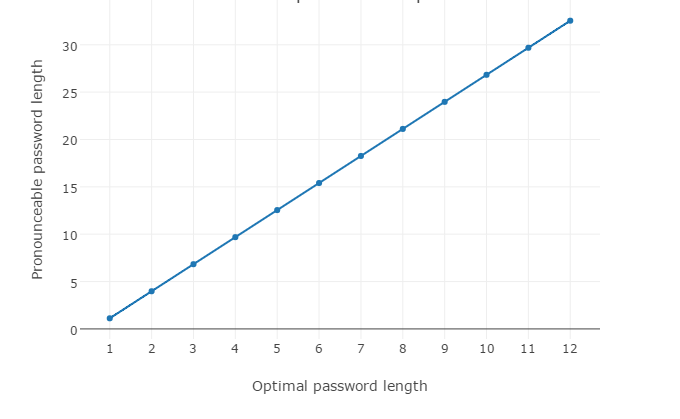
\includegraphics[width=0.5\linewidth]{figures/pronounceable}
  \caption{Pronounceable Password Space Size Comparison}
  \label{fig:pronounceable_password_space_size_comparison}
\end{figure}
\par The reduction in the password space was expected. On the other hand, this really only becomes a problem if the attacker knows for a fact that the password they are trying to crack is a pronounceable password. If they do not, they still have to try every other possible optimal password. Given that pronounceable passwords can be longer for the same difficulty in memorization, the reduction in space does not make pronounceable passwords not viable.

\subsection{Password Sharing}
\par An additional feature of this System is the means to share very sensitive information with other Users through password sharing. Suppose you need share your banking information with your accountant, whom you trust not to reveal it. There are few ways of doing so that are very secure. Vault5431 provides such a means. As was mentioned previously, the Client, at User creation, generates ElGamal keys and ECDSA keys. The Server, in this case, the Server as the PKI that distributes the keys associated with Users. The Client can trust that when it requests the public keys of a particular user, the Server is indeed responding with that User's key, since the Server signs and stores them securely. Therefore all the Client needs to do to send a password to a particular User is to request the User's public encryption key, encrypt the password under it and sign it with their private signing key. The Server adds this to the target User's shared password vault, which the target User can then view at their own leisure. They can then decide to save the password and add it to their own vault, or reject it.
\par In order to prevent Users from sharing infinitely many passwords with other Users, thereby bloating their shared password vault, a User $u$ may only have one shared password with another User $v$ at any given time. The Server will prevent further sharing from $u$ to $v$ until $v$ accepts $u$'s shared password. Also, the Client will automatically reject passwords whose signatures do not match.

\begin{thebibliography}{30}
  \bibitem{bib:session_storage}
    \url{https://developer.mozilla.org/en-US/docs/Web/API/Window/sessionStorage}
  \bibitem{bib:RFC7519}
    \url{https://www.ietf.org/rfc/rfc7519.txt}
  \bibitem{bib:TamperProof}
    \url{http://www.cs.cornell.edu/courses/cs5430/2016sp/l/11-logging/notes.html}
\end{thebibliography}

\end{document}
